\providecommand{\main}{..}		% Override relative path to the main file (already set in main file)
\documentclass[../InterneDSLs.tex]{subfiles}
\begin{document}

\chapter{Bau des Prototypen}

\section{Aufbau}
Die Verarbeitung der Grammatik erfolgt nach dem folgenden Schema:
\begin{itemize}
	\item Parsen der Grammatik
	\item Aufbau des Syntax-Baumes (aus Java-Typen)
	\item Abbildung in einen Graphen, der die Aufrufreihenfolge abbildet
	\item Generierung der Interfaces
\end{itemize}

\section{Parser}
Als Parser-Generator wurde ANTLR4 verwendet, der Parser zu einer EBNF-Grammatik in Java generieren kann. Dafür verwendet ANTLR aber eine unübliche Syntax, die sich an einer alten EBNF-Variante orientiert.

Der von ANTLR generierte Parser wird von einem Listener erweitert, der aus den EBNF-Konstrukten (die praktisch Strings entprechen) einen Baum aus eigenen Klassen generiert. Dadurch wird eine Typ-Sicherheit hergestellt, die durch die EBNF selbst nicht gegeben ist.

\section{Abbildung von EBNF auf Interfaces}
Zuerst wird die in EBNF geschriebene Grammatik in einen Baum aus Java-Objekten transformiert. Dadurch wird eine Typ-Sicherheit hergestellt und Methoden implementiert werden, die das Traversieren des Baumes vereinfachen. Abbildung~\ref{FIG:TypesBNF} zeigt die Typen und ihre Beziehungen untereinander. Diese Typen finden sich auch in den Regeln der EBNF-Grammatik (Abbildung~\ref{LST:EBNFGrammar}) wieder.

Danach wird aus dem Baum ein Graph generiert, der eine Abfolge aus Knoten und Kanten darstellt. Die Knoten repräsentieren die Scopes (die durchnummerierte Namen erhalten), die Kanten repräsentierten die Methoden. In den folgenden Abschnitten wird die Abbildung der EBNF-Konstrukte auf die des Graphen und Interfaces erklärt.

Zum Erstellen des Graphen wird die Bibliothek JGraphT\cite{JGraphT} verwendet. Sie bietet verschiedene Arten von Graphen aus der Graphentheorie mit dazugehörigen Algorithmen und Konsistenzregeln an. Die Bibliothek wird aktiv weiterentwickelt und benötigt Java ab Version 1.8.

Für diesen Anwendungsfall wird ein gerichteter Pseudo-Graph, der mehrere Kanten zwischen zwei Knoten erlaubt; mehrere Kanten werden bei optionalen Elementen und Schleifen benötigt.


\begin{figure}[ht]
\centering
\includegraphics[width=\linewidth]{\main/10_Pictures/BNF-Types}
\caption{Typen des BNF-Baumes}
\label{FIG:TypesBNF}
\end{figure}

\subsection{Kante mit einem Knoten}
Der einfachste Fall ist der von einer Sequenz, die nur ein Element beinhaltet. Hier kann das Element auf eine Kante zwischen zwei Knoten abgebildet werden. Die Namen der Scopes werden zu den Interfaces, bzw. zum Rückgabewert der Methode, deren Namen dem der der Kante entspricht. Grafik~\ref{FIG:OneElementNode} zeigt, wie eine Abbildung aussehen kann.
\begin{figure}[ht]
\centering
  \begin{subfigure}[c]{0.49\textwidth}
  	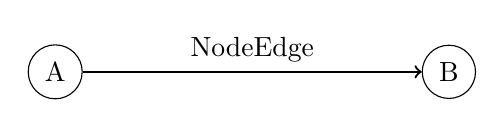
\begin{tikzpicture}
		\tikzset{vertex/.style = {shape=circle,draw,minimum size=.2em}}
		\tikzset{edge/.style = {->,> = latex'}}
		\node[vertex] (a) at  (0,0) {A};
		\node[vertex] (b) at  (5,0) {B};
		\path[->,draw,thick] (a) edge node[above] {NodeEdge} (b);
	\end{tikzpicture}
    \caption{Diagramm eines Sequenz-Knotens}
    \label{FIG:DiagramOneElementNode}
  \end{subfigure}
  \begin{subfigure}[c]{0.49\textwidth}
    \lstinputlisting[language=Java,caption={Java-Interface aus einem Sequenz-Knoten},label={LST:JInterfaceOneElementNode}]{Scope_one-element.java}
  \end{subfigure}
  \caption{Diagramm und Interface eines Sequenz-Knotens}
  \label{FIG:OneElementNode}
\end{figure}

\subsection{Sequenz von Knoten}
Tritt eine Sequenz von Knoten auf, muss für jeden Knoten ein Interface mit einer Methode generiert werden, um die Aufruf-Reihenfolge zu gewährleisten. Abbildung~\ref{FIG:SequenceNode} zeigt ein Beispiel mit zwei Knoten in einer Sequenz.
\begin{figure}[ht]
\centering
  \begin{subfigure}[c]{0.49\textwidth}
  	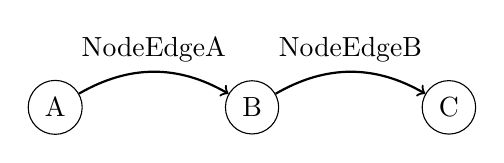
\begin{tikzpicture}
		\tikzset{vertex/.style = {shape=circle,draw,minimum size=.2em}}
		\tikzset{edge/.style = {->,> = latex'}}
		\node[vertex] (a) at  (0,0) {A};
		\node[vertex] (b) at  (2.5,0) {B};
		\node[vertex] (c) at  (5,0) {C};
		\path[->,draw,thick, bend left] (a) edge node[above] {NodeEdgeA} (b);
		\path[->,draw,thick, bend left] (b) edge node[above] {NodeEdgeB} (c);
	\end{tikzpicture}
    \caption{Diagramm einer Sequenz von Knoten}
    \label{FIG:DiagramSequenceNode}
  \end{subfigure}
  \begin{subfigure}[c]{0.49\textwidth}
    \lstinputlisting[language=Java,caption={Java-Interfaces aus einer Sequenz von Knoten},label={FIG:JInterfaceSequenceNode}]{Scope_sequence.java}
  \end{subfigure}
  \caption{Diagramm und Interface einer Sequenz von Knoten}
  \label{FIG:SequenceNode}
\end{figure}

\subsection{Kante mit Alternativen}
Alternativen in der EBNF können auf parallele Kanten vom selben Typ zwischen zwei Knoten abgebildet werden (siehe Abbildung~\ref{FIG:DiagramAlternativeNode}). Dadurch können beide Kanten analog wie bei einer Sequenz abgebildet werden, nur dass es einem Interface mehrere Methoden auftreten können (Listing~\ref{LST:JInterfaceAlternativeNode}). Die Interface-Typen und Rückgabewerte sind analog wie bei der Sequenz.
\begin{figure}[ht]
\centering
  \begin{subfigure}[c]{0.49\textwidth}
  	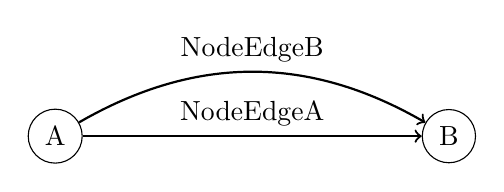
\begin{tikzpicture}
		\tikzset{vertex/.style = {shape=circle,draw,minimum size=.2em}}
		\tikzset{edge/.style = {->,> = latex'}}
		\node[vertex] (a) at  (0,0) {A};
		\node[vertex] (b) at  (5,0) {B};
		\path[->,draw,thick] (a) edge node[above] {NodeEdgeA} (b);
		\path[->,draw,thick, bend left] (a) edge node[above] {NodeEdgeB} (b);
	\end{tikzpicture}
    \caption{Diagramm alternativer Kanten}
    \label{FIG:DiagramAlternativeNode}
  \end{subfigure}
  \begin{subfigure}[c]{0.49\textwidth}
    \lstinputlisting[language=Java,caption={Java-Interface aus alternativen Kanten},label={LST:JInterfaceAlternativeNode}]{Scope_alternative.java}
  \end{subfigure}
  \caption{Diagramm und Interface alternativer Kanten}
  \label{FIG:AlternativeNode}
\end{figure}

\subsection{Optionales Element}
Im Falle eines optionalen Elementes, muss auch der Methodenaufruf optional sein und auch der nächstfolgende Methodenaufruf verfügbar sein. Das wird dadurch erreicht, indem das erste Interface vom folgenden erbt. Im Graphen wird das durch eine parallele Kante eines anderen Typen (OptionalEdge in Abbildung~\ref{FIG:DiagramOptionalNode}) repräsentiert. Listing~\ref{LST:JInterfaceOptionalNode}) ist, bis auf die Vererbung, gleich zu Listing~\ref{LST:JInterfaceOneElementNode}.
\begin{figure}[ht]
\centering
  \begin{subfigure}[c]{0.49\textwidth}
  	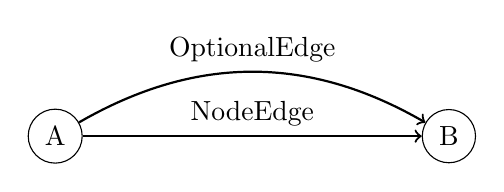
\begin{tikzpicture}
		\tikzset{vertex/.style = {shape=circle,draw,minimum size=.2em}}
		\tikzset{edge/.style = {->,> = latex'}}
		\node[vertex] (a) at  (0,0) {A};
		\node[vertex] (b) at  (5,0) {B};
		\path[->,draw,thick] (a) edge node[above] {NodeEdge} (b);
		\path[->,draw,thick, bend left] (a) edge node[above] {OptionalEdge} (b);
	\end{tikzpicture}
    \caption{Diagramm einer optionalen Kante}
    \label{FIG:DiagramOptionalNode}
  \end{subfigure}
  \begin{subfigure}[c]{0.49\textwidth}
    \lstinputlisting[language=Java,caption={Java-Interface aus einer optionalen Kante},label={LST:JInterfaceOptionalNode}]{Scope_optional.java}
  \end{subfigure}
  \caption{Diagramm und Interface einer optionalen Kante}
  \label{FIG:OptionalNode}
\end{figure}

\subsection{Kante mit optionaler Schleife}
Da die Wiederholung bei EBNF optional ist (beliebig oft oder keinmal auftreten darf), gibt es hier, wie beim optionalen Element eine Kante vom Typ OptionalEdge. Dadurch kann der Methodenaufruf übersprungen werden.

Um den Methodenaufruf wiederholbar zu machen kann man nicht einfach eine parallele, optionale Kante in die entgegengesetzte Richtung einfügen, weil diese ebenfalls in eine Vererbung umgesetzt würde; dadurch würde zwischen beiden Interfaces eine zirkuläre Abhängigkeit entstehen, die in Java verboten ist.

Stattdessen wird bei der optionalen Wiederholung die Kante, die den Methodenaufruf repräsentiert, eine Schleife zum Knoten selbst. Somit kann die Methode beliebig oft aufgerufen werden, bevor die in B deklarierte Methode aufgerufen wird (Abbildung~\ref{FIG:DiagramLoopNode}).
\begin{figure}[ht]
\centering
  \begin{subfigure}[c]{0.49\textwidth}
  	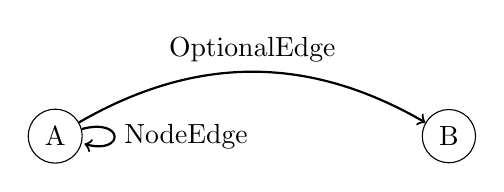
\begin{tikzpicture}
		\tikzset{vertex/.style = {shape=circle,draw,minimum size=.2em}}
		\tikzset{edge/.style = {->,> = latex'}}
		\node[vertex] (a) at  (0,0) {A};
		\node[vertex] (b) at  (5,0) {B};
		\path[->,draw,thick, bend left] (a) edge node[above] {OptionalEdge} (b);
		\path[->,draw,thick, loop right] (a) edge node[right] {NodeEdge} (a);
	\end{tikzpicture}
    \caption{Diagramm einer Schleifen-Kante (Variante 1)}
    \label{FIG:DiagramLoopNode}
  \end{subfigure}
  \begin{subfigure}[c]{0.49\textwidth}
    \lstinputlisting[language=Java,caption={Java-Interface aus einer Schleifen-Kante (Variante 1)},label={LST:JInterfaceLoopNode}]{Scope_loop.java}
  \end{subfigure}
  \caption{Diagramm und Interface einer Schleifen-Kante (Variante 1)}
  \label{FIG:LoopNode}
\end{figure}

Eine Alternative zur Schleifen-Kante am ersten Scope ist eine am zweiten Scope (Abbildung~\ref{FIG:DiagramLoopNodeAlternative}); hier kann der Methodenaufruf ebenfalls übersprungen werden, indem die Methoden der anderen ausgehenden Kanten aufgerufen werden oder beliebig oft, da der selbe Scope zurückgegeben wird.
\begin{figure}[ht]
\centering
  \begin{subfigure}[c]{0.49\textwidth}
  	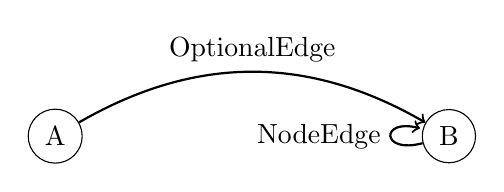
\begin{tikzpicture}
		\tikzset{vertex/.style = {shape=circle,draw,minimum size=.2em}}
		\tikzset{edge/.style = {->,> = latex'}}
		\node[vertex] (a) at  (0,0) {A};
		\node[vertex] (b) at  (5,0) {B};
		\path[->,draw,thick, bend left] (a) edge node[above] {OptionalEdge} (b);
		\path[->,draw,thick, loop left] (b) edge node[left] {NodeEdge} (b);
	\end{tikzpicture}
    \caption{Diagramm einer Schleifen-Kante (Variante 2)}
    \label{FIG:DiagramLoopNodeAlternative}
  \end{subfigure}
  \begin{subfigure}[c]{0.49\textwidth}
    \lstinputlisting[language=Java,caption={Java-Interface aus einer Schleifen-Kante (Variante 2)},label={LST:JInterfaceLoopNodeAlternative}]{Scope_loop_alt.java}
  \end{subfigure}
  \caption{Diagramm und Interface einer Schleifen-Kante (Variante 2)}
  \label{FIG:LoopNodeAlternative}
\end{figure}

Eine dritte Möglichkeit besteht darin, die bei dem Verschachteln der Konstrukte wieder aufgegriffen wird, ist ein zusätzlicher Knoten, der zum nächsten und vorherigen Knoten mit je einer optionalen Kante verbunden ist (siehe Abblindung~\ref{FIG:DiagramLoopNodeAlternativeTwo}). Die Methoden aud C werden in A und B aufrufbar gemacht, wodurch der Aufruf an NodeEdge optional und mehrfach aufrufbar gemacht wird.
\begin{figure}[ht]
\centering
  \begin{subfigure}[c]{0.49\textwidth}
  	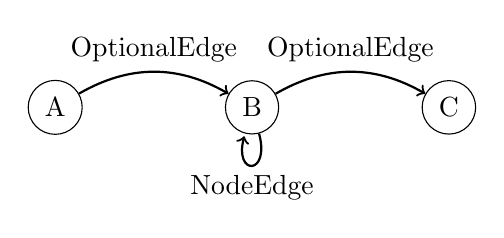
\begin{tikzpicture}
		\tikzset{vertex/.style = {shape=circle,draw,minimum size=.2em}}
		\tikzset{edge/.style = {->,> = latex'}}
		\node[vertex] (a) at  (0,0) {A};
		\node[vertex] (b) at  (2.5,0) {B};
		\node[vertex] (c) at  (5,0) {C};
		\path[->,draw,thick, bend left] (a) edge node[above] {OptionalEdge} (b);
		\path[->,draw,thick, loop below] (b) edge node[below] {NodeEdge} (b);
		\path[->,draw,thick, bend left] (b) edge node[above] {OptionalEdge} (c);
	\end{tikzpicture}
    \caption{Diagramm einer Schleifen-Kante (Variante 3)}
    \label{FIG:DiagramLoopNodeAlternativeTwo}
  \end{subfigure}
  \begin{subfigure}[c]{0.49\textwidth}
    \lstinputlisting[language=Java,caption={Java-Interface aus einer Schleifen-Kante (Variante 3)},label={LST:JInterfaceLoopNodeAlternativeTwo}]{Scope_loop_alt_two.java}
  \end{subfigure}
  \caption{Diagramm und Interface einer Schleifen-Kante (Variante 3)}
  \label{FIG:LoopNodeAlternativeTwo}
\end{figure}

Eine vierte Möglichkeit besteht darin, die drei Knoten aus Variante 3 (Abbildung~\ref{FIG:DiagramLoopNodeAlternativeTwo}) zusammenzuführen.

\subsection{Schachtelung der Konstrukte}
In diesem Abschnitt wird darauf eingegangen, wie die Rekursion der ENBF-Konstrukte behandelt werden können. Die Fälle von Alternative und Schleifen in einer Sequenz werden aus Trivialität übersprungen. Hier soll nur auf Fälle eingegangen werden, die nicht aus den vorherigen Beispielen ersichtlich sind.

\subsubsection{Sequenz in einer Schleife}
Befindet sich eine Sequenz in einer Schleife, bilden die Knoten und Kanten eine Schleife zum Ziel-Knoten (Abbildung~\ref{FIG:DiagramSequenceInLoop}) der Schleife analog zur zweiten Variante der Schleife (siehe Abbildung~\ref{FIG:DiagramLoopNodeAlternative}).
\begin{figure}[ht]
\centering
  \begin{subfigure}[c]{0.49\textwidth}
  	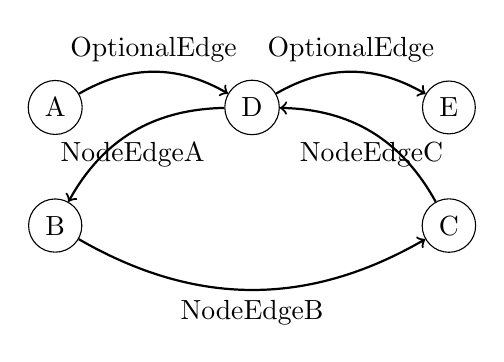
\begin{tikzpicture}
		\tikzset{vertex/.style = {shape=circle,draw,minimum size=.2em}}
		\tikzset{edge/.style = {->,> = latex'}}
		\node[vertex] (a) at  (0,1.5) {A};
		\node[vertex] (b) at  (0,0) {B};
		\node[vertex] (c) at  (5,0) {C};
		\node[vertex] (d) at  (2.5,1.5) {D};
		\node[vertex] (e) at  (5,1.5) {E};
		\path[->,draw,thick, bend left] (a) edge node[above] {OptionalEdge} (d);
		\path[->,draw,thick, bend left] (d) edge node[above] {OptionalEdge} (e);
		\path[->,draw,thick, bend right] (d) edge node[below] {NodeEdgeA} (b);
		\path[->,draw,thick, bend right] (b) edge node[below] {NodeEdgeB} (c);
		\path[->,draw,thick, bend right] (c) edge node[below] {NodeEdgeC} (d);
	\end{tikzpicture}
    \caption{Diagramm einer Sequenz innerhalb eines Schleifen-Knotens}
    \label{FIG:DiagramSequenceInLoop}
  \end{subfigure}
  \begin{subfigure}[c]{0.49\textwidth}
    \lstinputlisting[language=Java,caption={Java-Interface aus einer Sequenz in einem Schleifen-Knoten},label={LST:JInterfaceSequenceInLoop}]{Sequence_in_loop.java}
  \end{subfigure}
  \caption{Diagramm und Interface einer Sequenz innerhalb eines Schleifen-Knotens (nach Variante 2)}
  \label{FIG:SequenceInLoop}
\end{figure}

\subsubsection{Alternative in einer Schleife}
Befindet sich eine Alternative in einer Schleife, werden alle Alternativen, die nur aus einer Kante bestehen, in eine Schleifen-Kante am Ziel-Knoten der Schleife transformiert. Besteht eine Alternative aus einer Sequenz, wird aus dieser Sequenz eine weitere Schleife aus mehreren Kanten und Knoten.

Falls die Alternative sich in einer Sequenz in einer Alternative befindet, gibt es in der Schleife mehrere ausgehende Kanten vom Ziel-Knoten der Schleife (siehe Abbildung~\ref{FIG:DiagramAlternativeInLoop}).
\begin{figure}[ht]
\centering
  \begin{subfigure}[c]{0.49\textwidth}
  	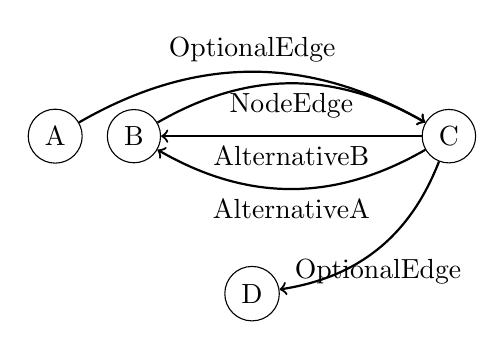
\begin{tikzpicture}
		\tikzset{vertex/.style = {shape=circle,draw,minimum size=.2em}}
		\tikzset{edge/.style = {->,> = latex'}}
		\node[vertex] (a) at  (0,0) {A};
		\node[vertex] (b) at  (1,0) {B};
		\node[vertex] (c) at  (5,0) {C};
		\node[vertex] (d) at  (2.5,-2) {D};
		\path[->,draw,thick, bend left] (a) edge node[above] {OptionalEdge} (c);
		\path[->,draw,thick, bend left] (c) edge node[below] {OptionalEdge} (d);
		\path[->,draw,thick, bend left] (c) edge node[below] {AlternativeA} (b);
		\path[->,draw,thick] (c) edge node[below] {AlternativeB} (b);
		\path[->,draw,thick, bend left] (b) edge node[below] {NodeEdge} (c);
	\end{tikzpicture}
    \caption{Diagramm einer Alternative und Sequenz innerhalb eines Schleifen-Knotens}
    \label{FIG:DiagramAlternativeInLoop}
  \end{subfigure}
  \begin{subfigure}[c]{0.49\textwidth}
    \lstinputlisting[language=Java,caption={Java-Interface aus einem Schleifen-Knoten},label={LST:JInterfaceAlternativeInLoop}]{Loop_with_inner_alternative_and_sequence.java}
  \end{subfigure}
  \caption{Diagramm und Interface einer Alternative und Sequenz innerhalb eines Schleifen-Knotens (nach Variante 2)}
  \label{FIG:AlternativeInLoop}
\end{figure}

\subsubsection{Schleife in Alternative}
Befindet sich eine Schleife in einer Alternative, muss für ihre Kante ein Hilfsknoten eingeführt werden, auch wenn die Schleife nur eine Kante beinhaltet (Knoten C in Abbildung~\ref{FIG:DiagramLoopInAlternative}). Würde man die optionalen Kante direkt von A nach B aufnehmen, wären NodeEdgeB und NodeEdgeC ebenfalls optional und würde nicht dem EBNF-Konstrukt entsprechen.
\begin{figure}[ht]
\centering
  \begin{subfigure}[c]{0.49\textwidth}
  	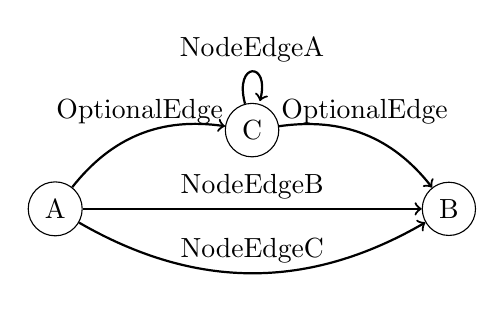
\begin{tikzpicture}
		\tikzset{vertex/.style = {shape=circle,draw,minimum size=.2em}}
		\tikzset{edge/.style = {->,> = latex'}}
		\node[vertex] (a) at  (0,0) {A};
		\node[vertex] (b) at  (5,0) {B};
		\node[vertex] (c) at  (2.5,1) {C};
		\path[->,draw,thick, bend left] (a) edge node[above] {OptionalEdge} (c);
		\path[->,draw,thick, bend left] (c) edge node[above] {OptionalEdge} (b);
		\path[->,draw,thick, loop above] (c) edge node[above] {NodeEdgeA} (c);
		\path[->,draw,thick] (a) edge node[above] {NodeEdgeB} (b);
		\path[->,draw,thick, bend right] (a) edge node[above] {NodeEdgeC} (b);
	\end{tikzpicture}
    \caption{Diagramm einer Schleife innerhalb einer Alternative}
    \label{FIG:DiagramLoopInAlternative}
  \end{subfigure}
  \begin{subfigure}[c]{0.49\textwidth}
    \lstinputlisting[language=Java,caption={Java-Interface aus einer Schleife innerhalb einer Alternative},label={LST:JInterfaceLoopInAlternative}]{Loop_with_inner_alternative_and_sequence.java}
  \end{subfigure}
  \caption{Diagramm und Interface einer Schleife innerhalb einer Alternative}
  \label{FIG:LoopInAlternative}
\end{figure}


\section{Schwierigkeiten beim Bau}
Beim Erstellen des Prototypen traten einige Schwierigkeiten auf. Die größten werden in diesem Abschnitt besprochen: die Behandlung der Rekursion der EBNF-Grammatik und die der Typen.

\subsection{Behandlung der Rekursion}

\subsection{Typen}

\subsubsection{Mapping auf Typen der Hostsprache}
- NTs -> Methoden (Einschränungen)

- Interfacenamen beliebig

\subsubsection{Generierung von Typen aus EBNF-Regeln}


\section{Einschränkungen bei der Grammatik}
Die EBNF-Grammatik kann nicht beliebig formuliert sein.

\subsection{Startregel}
In der Grammatik muss eine Startregel definiert sein, die nur ein Nicht-Terminal beinhaltet. Daraus wird das erste Interface als Einstiegspunkt generiert.

\subsection{Lexer-Regeln}
Für jede Lexer-Regel sollte es eine entsprechende Parser-Regel geben, die nur die jeweilige Lexer-Regel beinhaltet. Dadurch kann der Listener des Parsers die Typen auch verarbeiten.

Falls eine Regel innerhalb einer anderen vorkommt, ohne ein Trennsymbol zu einer anderen, darf es ebenfalls keine Lexer-Regel sein, um vom Listener erkannt zu werden.


\chapter{Testlauf mit anschaulichem Beispiel}


\section{Optimierungspotenzial}


\section{Varianten}


\end{document}
